\documentclass[10pt, xcolor=dvipsnames, handout]{beamer}
\usepackage[utf8]{inputenc}
\usetheme{metropolis}
\setbeamercolor{frametitle}{fg=Black,bg=White}
\setbeamercolor{background canvas}{bg=White}
\usepackage{biblatex}
\addbibresource{BT_final_refs.bib}
\usepackage{graphicx}
\usepackage{subcaption}
\usepackage{physics}
\usepackage{hyperref}
\title{How Can Organisations Innovate?}

\date{18 June 2018}
\author{Ambrose Yim, supervised by Stephen Cassidy, Stephen Brewis (BT); Renaud Lambiotte, Andrew Mellor (Oxford)}
\institute{InFoMM CDT, Mathematical Institute, University of Oxford}

\begin{document}

\maketitle

\begin{frame}{Motivation}

We want to understand the conditions for agents in an organisation to cooperate.

\pause Can a small fraction of `innovators' in the system influence the entire population to adopt a new idea?

\pause What is the interplay between the population's \textbf{willingness} to accept new behaviour and the way they \textbf{communicate}?

\pause What if there are \textbf{constraints} that agents are not aware of?
\end{frame}

\begin{frame}{What we will learn today}
Segregating agents into individual teams hinder innovation if new problems come up that require agents across teams to coordinate.

\pause Duh!
\end{frame}

\begin{frame}{Model}
Key modelling assumptions:
\begin{itemize}
\pause \item Agents are connected in a \textbf{social network} \cite{wang_social_2018} \cite{granell_dynamical_2013}
\pause \item Each agent receives \emph{information} via its social network
\pause \item An agent's decision making is \emph{constrained} by the decisions of other agents (\textbf{dependency network})
\end{itemize}

\end{frame}

\begin{frame}

\begin{figure}[htb]
\includegraphics[width=0.9\textwidth]{figures/multiplex.jpeg}
\end{figure}
\end{frame}

\begin{frame}{Agent behaviour}
What is an agent? How do they coordinate? \cite{granell_dynamical_2013}
\begin{itemize}
\pause \item Each agent has two states: default (0) or innovate (1)
\pause \item All agents start in the default state.
\pause \item Suppose there is a problem in the organisation that can only be solved if \emph{all} agents coordinate.
\end{itemize}
\end{frame}



\begin{frame}{Agent behaviour}
\begin{itemize}
\pause \item If too few neighbours on the dependency network decide to innovate, then it is not favourable for an agent to innovate
\pause \item Each agent has a \textbf{dependency threshold}: number of innovating dependency neighbours for it to `see' the benefit of innovation
\end{itemize}
\end{frame}

\begin{frame}{Agent behaviour}
In game theory language, we say the agents play a \textbf{coordination game} (a.k.a. \textbf{Prisoners' Dilemma}) \cite{shoham_multiagent_2008} \cite{jackson_games_2014}.
\begin{itemize}
\pause \item \textbf{positive pay-off} if it innovates \emph{and} sufficiently many of its dependency neighbours innovate
\pause \item \textbf{negative pay-off} if it innovates \emph{but} not enough agents that constrain you decide with innovate
\pause \item \textbf{neutral pay-off} if it remains in the default state.
\end{itemize}
We assume dependency is reflexive; if A influences B then B influences A.
\end{frame}

\begin{frame}{Agent behaviour}
\begin{itemize}
\pause \item Agents must first be \emph{aware} of innovation via their social network
\pause \item Agents have varying `social awareness': number of `friends` required to persuade you to adopt new ideas
\end{itemize}
\end{frame}

\begin{frame}[standout]
Agents must be aware and receive a positive pay-off from innovation to change its state from default to innovation.
\end{frame}

\begin{frame}{Network Construction}
\begin{itemize}
\pause \item Initially, we assume social network $\mathcal{S}$ = dependency network $\mathcal{D}$
\pause \item Over time the business environment changes
\pause \item If not updated timely, $\mathcal{S}\neq \mathcal{D}$
\end{itemize}
\end{frame}
\begin{frame}{Network Construction}
\pause We study two modes of `information degradation' $\mathcal{S}\to \mathcal{D}$ \cite{brummitt_multiplexity-facilitated_2012}
\begin{enumerate}
\pause \item Random edge swap:
  \begin{itemize}
  \pause \item $a-b$ and $c- d$ $\Rightarrow$ $a -d$ and $c- b$.
  \pause \item Agents preserve their degree (number of neighbours) from $\mathcal{S} \to \mathcal{D}$
  \pause \item Network topology (neighbourhood relations) is \emph{altered} (loose memory of neighbours).
  \end{itemize}
\pause \item Random node reshuffle:
\begin{itemize}
\pause \item Agent degree in $\mathcal{D} \neq$ degree in $\mathcal{S}$.
\pause \item Network topology is \emph{preserved} (but loose memory of position in network).
\pause \item In random degree distribution networks, same as rewiring edges.
\end{itemize}
\end{enumerate}
\end{frame}

\begin{frame}{Random Network Classes}

Random graphs with nodes sampled from a degree distribution then randomly connected.
\begin{enumerate}
\pause \item Erdős-Rényi Graph \cite{erdos_random_1959} \cite{newman_random_2001}
\begin{itemize}
\item Each pair of nodes has a probability $p$ of forming an edge.
\pause \item Average degree $z = Np$. Degree distribution is Binomial.
\end{itemize}
\pause \item `Planted Partition Model'\cite{karrer_stochastic_2011}
\begin{itemize}
\item Agents are segregated into $C$ \textbf{communities} of equal size $n$.
\pause \item Between pairs of nodes in the same community there is a probability $p_i$ of forming an edge.
\pause \item Between pairs of nodes in different communities there is a probability $p_o$ of forming an edge.
\pause \item Average degree $z = (n-1)p_i + (C-1)np_o$.
\pause \item We fix $C=100$ and $n=100$, with $(C-1)np_o = 1/2$.
\end{itemize}
\end{enumerate}
\end{frame}


\begin{frame}{Thresholds}
We assume social threshold and dependency thresholds are independent. \cite{lee_threshold_2014}

\pause We define the social/dependency threshold  = fraction of neighbours above which node becomes aware/susceptible to infection

\begin{enumerate}
\pause \item Agent randomly samples both thresholds independently from the same normal distribution (vary mean $r$ and fix $\sigma = 0.2$) \cite{gleeson_seed_2007}
\pause \item Dependency threshold sampled from normal distribution but social threshold = if one friend is innovating agent is aware.
\end{enumerate}

Agents with a \emph{negative} dependency and social thresholds are \emph{innovators} who would innovate no matter what.

\end{frame}

\begin{frame}[standout]
social network $\otimes$ social threshold $\otimes$ dependency layer $\otimes$ dependency threshold.
\end{frame}

\begin{frame}{Single layer analysis: Watts-Gleeson Theory}

Consider social layer = dependency layer and the thresholds are identical for each node.

\pause Watts-Gleeson theory \cite{watts_simple_2002} \cite{gleeson_seed_2007} applies to infinite random graphs with negligible clustering (probability of three connected nodes forming a triangle $\to 0$ as $N \to \infty$), or being \emph{locally tree like}.

\pause We can think of this process of synchronously updating the state of nodes as an \textbf{infection} from infinitely far away in the network.

\end{frame}

\begin{frame}{Single layer analysis: Watts-Gleeson Theory}

\begin{figure}[htb]
\includegraphics[width=0.8\textwidth]{figures/tree.png}
\end{figure}

\end{frame}

\begin{frame}{Single layer analysis: Watts-Gleeson Theory}

\begin{figure}[htb]
\includegraphics[width=0.4\textwidth]{figures/tree.png}
\end{figure}

Initially all nodes are in the 0 state. Infection initiated on level $n=0$ at time $t=0$.

{\pause Probability that a node on layer $n+1$ is infected at time $n+1$ is dependent on the fraction of nodes infected in layer $n$:
\begin{equation}
q_{n+1} = g(q_n\ ; r)
\end{equation}
}


\end{frame}

\begin{frame}{Single layer analysis: Watts-Gleeson Theory}

\begin{figure}[htb]
\includegraphics[width=0.4\textwidth]{figures/tree.png}
\end{figure}

\pause Brouwer fixed point theorem: there exists $q = g(q\ ; r)$. Fixed point is either stable or unstable.

\pause Final layer must be a (stable) fixed point. Let $q_\infty = \Pr(\text{infection on final layer} \ | \ \text{top node inactive})$.

\pause Final fraction of infected nodes is
\begin{equation}
\rho = \rho(q_\infty\ ; r)
\end{equation}

\end{frame}

\begin{frame}{Single layer analysis: Watts-Gleeson Theory}
We look at Erdős-Rényi graphs of varying mean degree.
\begin{figure}[htb]
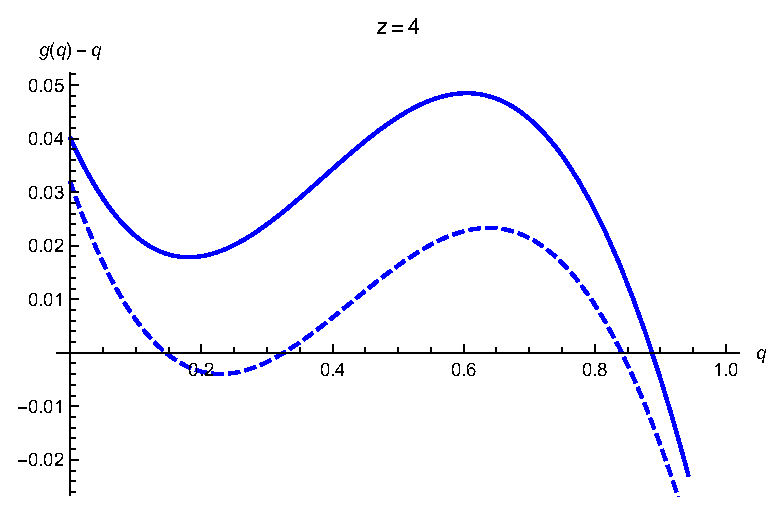
\includegraphics[width=0.8\textwidth]{figures/single_layer_gq}
\caption{$g(q)-q$ for parameters $z=4$;  sold is $r=0.35$, dashed is $r=0.371$}
\end{figure}

\end{frame}
\begin{frame}{Single layer analysis: Watts-Gleeson Theory}
\begin{figure}
    \centering
    \begin{subfigure}[b]{0.4\textwidth}
        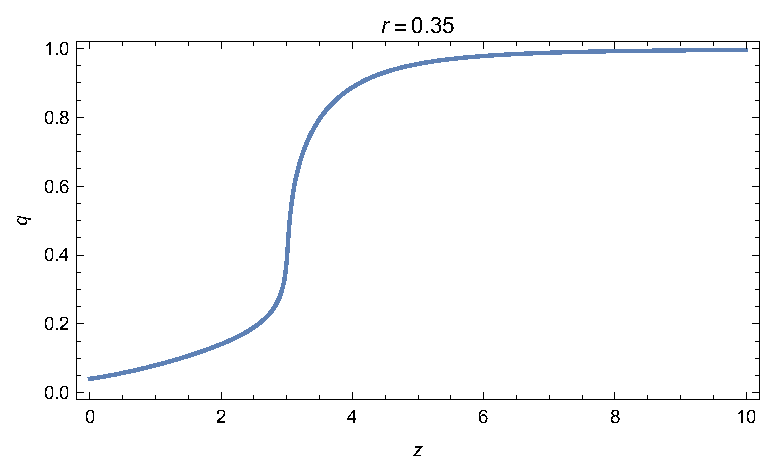
\includegraphics[width=\textwidth]{figures/one_layer_qz_r035}
    \end{subfigure}
    ~ %add desired spacing between images, e. g. ~, \quad, \qquad, \hfill etc.
      %(or a blank line to force the subfigure onto a new line)
    \begin{subfigure}[b]{0.4\textwidth}
        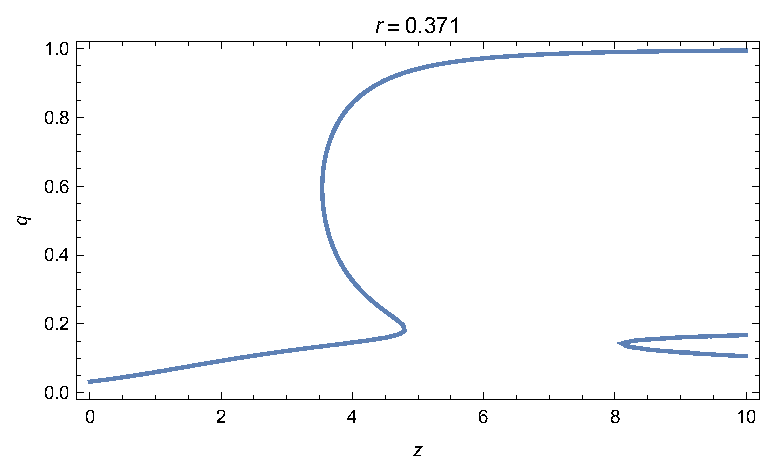
\includegraphics[width=\textwidth]{figures/one_layer_qz_r0371}
    \end{subfigure}
    ~ %add desired spacing between images, e. g. ~, \quad, \qquad, \hfill etc.
    %(or a blank line to force the subfigure onto a new line)
    \begin{subfigure}[b]{0.4\textwidth}
        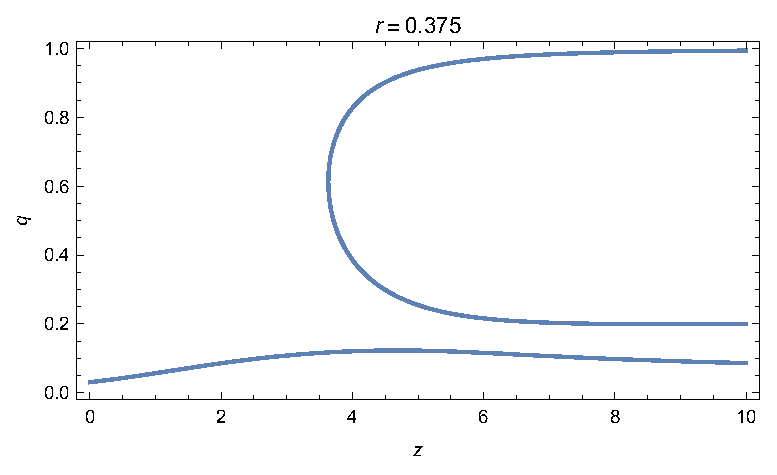
\includegraphics[width=\textwidth]{figures/one_layer_qz_r0375}
    \end{subfigure}
    \caption{Fixed point plot for increasing $r$. Note Goldilocks zone in middle figure.}
\end{figure}
\end{frame}

\begin{frame}{Single layer analysis: Watts-Gleeson Theory}
\begin{figure}
    \centering
    \begin{subfigure}[b]{0.4\textwidth}
        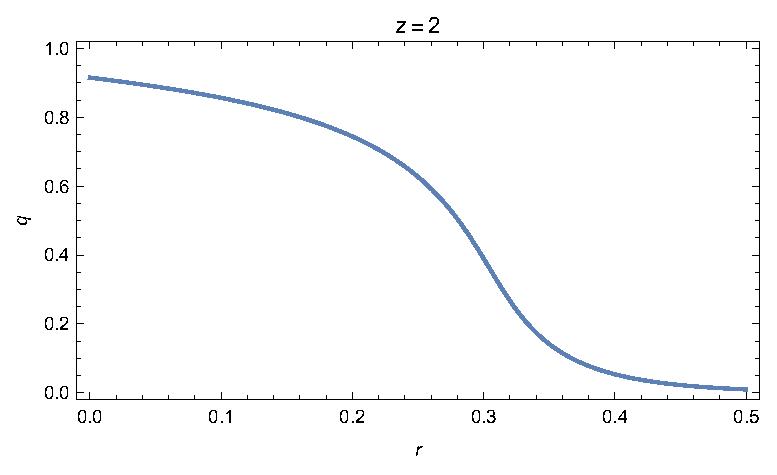
\includegraphics[width=\textwidth]{figures/one_layer_qr_z2}
    \end{subfigure}
    ~ %add desired spacing between images, e. g. ~, \quad, \qquad, \hfill etc.
      %(or a blank line to force the subfigure onto a new line)
    \begin{subfigure}[b]{0.4\textwidth}
        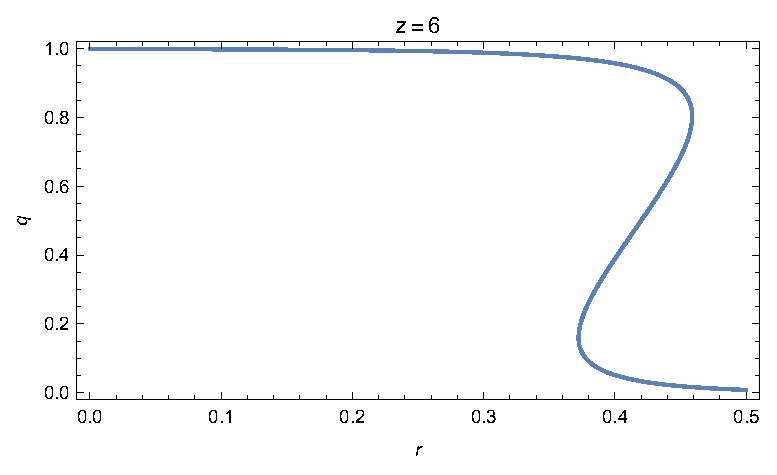
\includegraphics[width=\textwidth]{figures/one_layer_qr_z6}
    \end{subfigure}
    ~ %add desired spacing between images, e. g. ~, \quad, \qquad, \hfill etc.
    %(or a blank line to force the subfigure onto a new line)
    \caption{Fixed point plot for increasing $z$.}
\end{figure}
\end{frame}

\begin{frame}{Single layer analysis: Watts-Gleeson Theory}
First and Second order (approximate) cascade conditions: $(z,r)$ values that induces a global cascade of infection contained in the union of both regions.
\begin{figure}
\centering
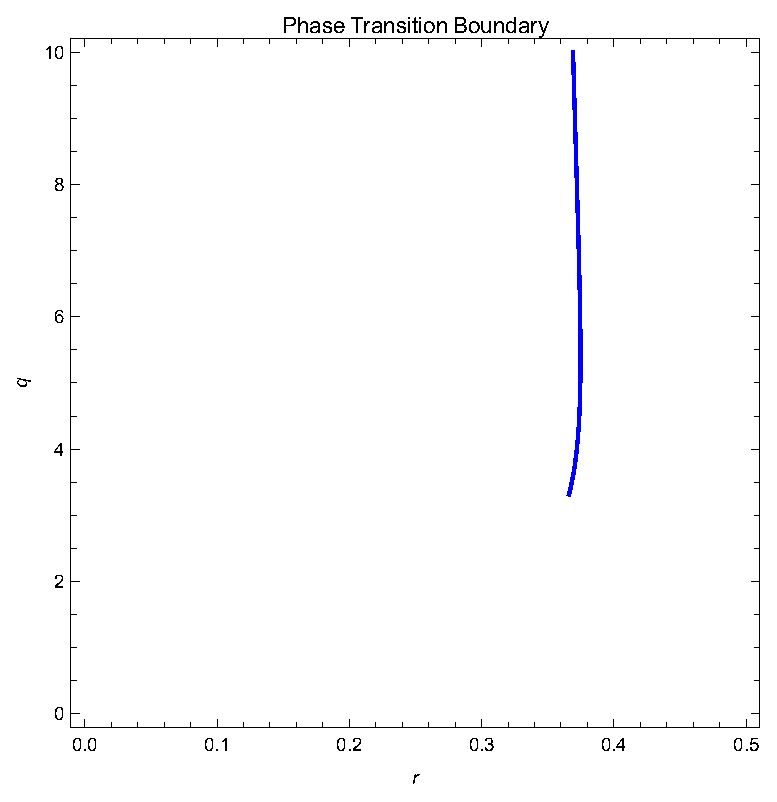
\includegraphics[width=0.5\textwidth]{figures/single_layer_cascade}
\end{figure}
\end{frame}


\begin{frame}{Double layer analysis: Watts-Gleeson Theory}
Technically need two $q$ probabilities for the two different layers respectively; however agent randomly samples both thresholds independently from the \emph{same} normal distribution, so symmetry reduces the system to one variable.

\begin{figure}
    \centering
    \begin{subfigure}[b]{0.435\textwidth}
        \includegraphics[width=\textwidth]{figures/edge_swap_zr}
    \end{subfigure}
    ~ %add desired spacing between images, e. g. ~, \quad, \qquad, \hfill etc.
      %(or a blank line to force the subfigure onto a new line)
    \begin{subfigure}[b]{0.4\textwidth}
        \includegraphics[width=\textwidth]{figures/node_swap_zr}
    \end{subfigure}
    ~ %add desired spacing between images, e. g. ~, \quad, \qquad, \hfill etc.
    %(or a blank line to force the subfigure onto a new line)
    \caption{Final fraction size vs $(z,r)$; white curve second order cascade condition}
\end{figure}

\end{frame}

\begin{frame}{Double layer analysis: Watts-Gleeson Theory}
\begin{figure}
    \centering
    \begin{subfigure}[b]{0.4\textwidth}
        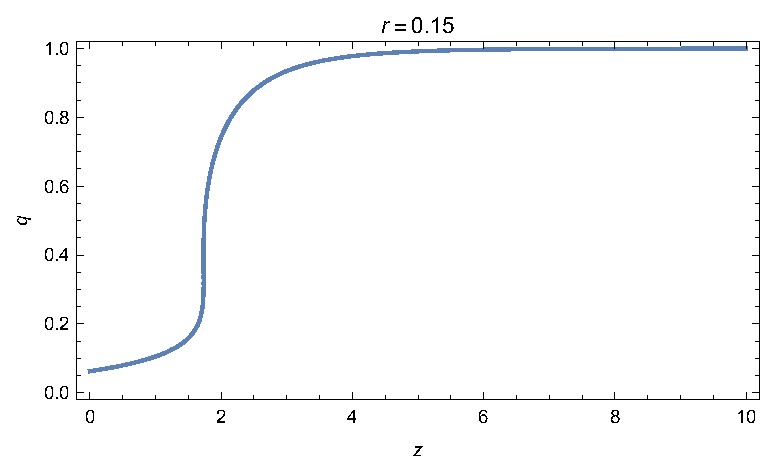
\includegraphics[width=\textwidth]{figures/two_layer_edge_qz_r015}
    \end{subfigure}
    ~ %add desired spacing between images, e. g. ~, \quad, \qquad, \hfill etc.
      %(or a blank line to force the subfigure onto a new line)
    \begin{subfigure}[b]{0.4\textwidth}
        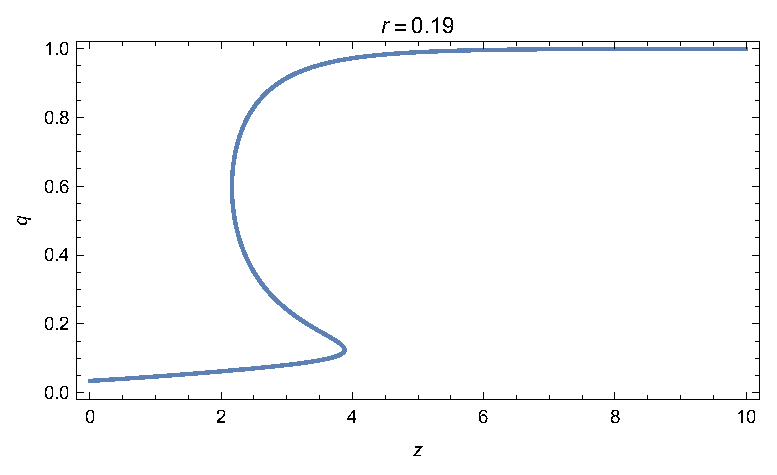
\includegraphics[width=\textwidth]{figures/two_layer_edge_qz_r019}
    \end{subfigure}
    ~ %add desired spacing between images, e. g. ~, \quad, \qquad, \hfill etc.
    %(or a blank line to force the subfigure onto a new line)
    \begin{subfigure}[b]{0.4\textwidth}
        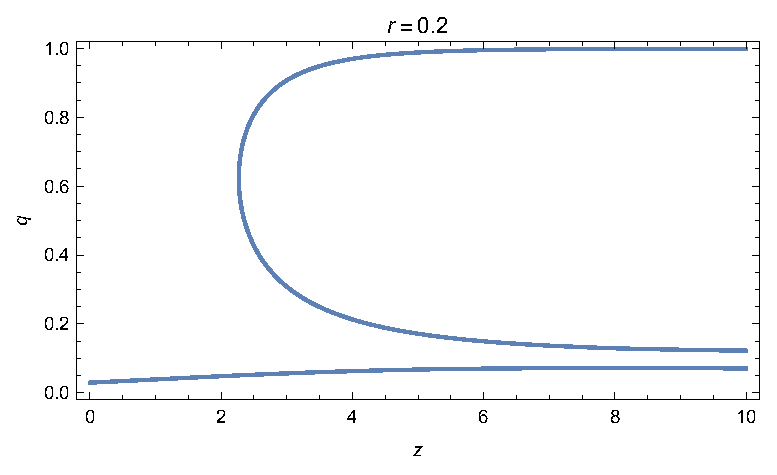
\includegraphics[width=\textwidth]{figures/two_layer_edge_qz_r02}
    \end{subfigure}
    ~
    \caption{Edge swap: Fixed points cross section across different $r$ values. Note that the Goldilocks zone disappears. }
\end{figure}
\end{frame}

\begin{frame}{Double layer analysis: Watts-Gleeson Theory}
\begin{figure}
    \centering
    \begin{subfigure}[b]{0.4\textwidth}
        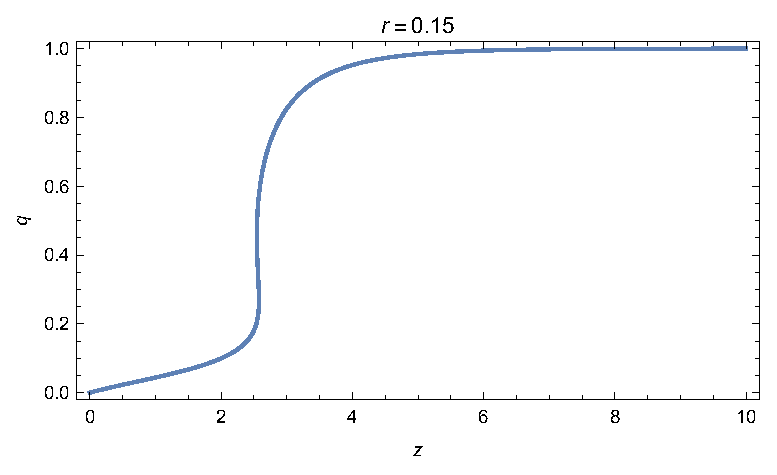
\includegraphics[width=\textwidth]{figures/two_layer_node_qz_r015}
    \end{subfigure}
    ~ %add desired spacing between images, e. g. ~, \quad, \qquad, \hfill etc.
      %(or a blank line to force the subfigure onto a new line)
    \begin{subfigure}[b]{0.4\textwidth}
        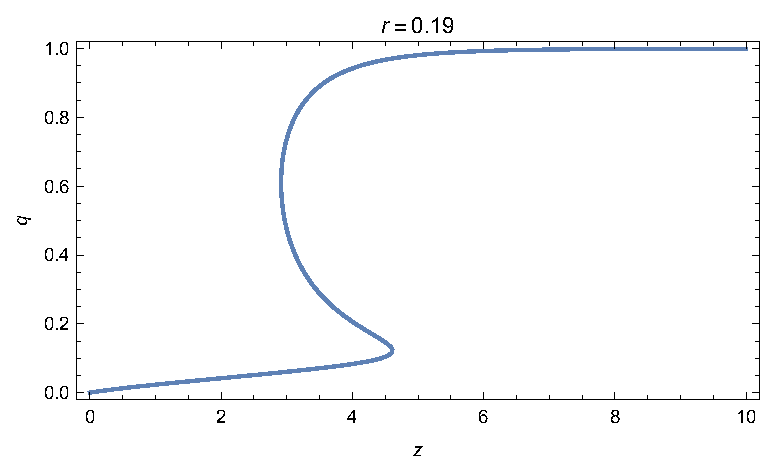
\includegraphics[width=\textwidth]{figures/two_layer_node_qz_r019}
    \end{subfigure}
    ~ %add desired spacing between images, e. g. ~, \quad, \qquad, \hfill etc.
    %(or a blank line to force the subfigure onto a new line)
    \begin{subfigure}[b]{0.4\textwidth}
        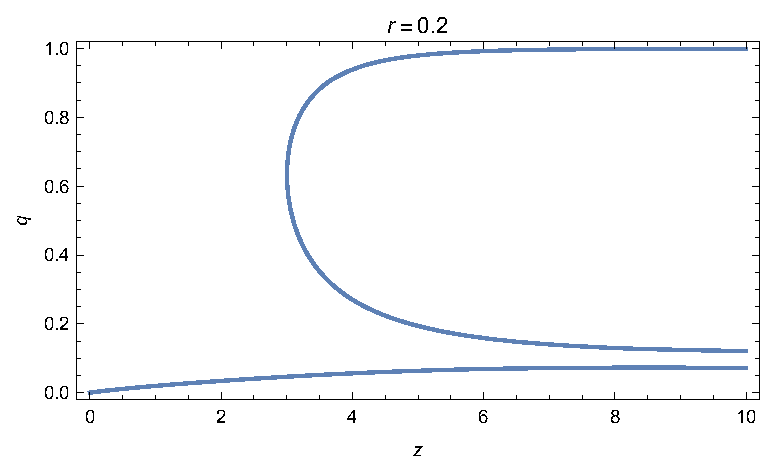
\includegraphics[width=\textwidth]{figures/two_layer_node_qz_r02}
    \end{subfigure}
    ~
    \caption{Node swap: Fixed points cross section across different $r$ values. Note that the Goldilocks zone disappears. }
\end{figure}
\end{frame}

\begin{frame}{Summary of Analytical Results}
\begin{itemize}
\pause \item The final infection size decreases as $r$ increases
\pause \item The transition becomes steeper and steeper as $z$ increases
\pause \item Transition becomes \emph{discontinuous} for values of $r$ and $z$ greater than some critical value.
\pause \item Discontinuous transition separates two `phases' where the global cascade is extensive across the population and the other where the infection does not spread.
\pause \item Adding an extra layer lowers the critical value of $r$ where the discontinuity takes place.
\pause \item In single layer, there is a competition between the benefits of increasing node degree to increase the chance of exposure vs the increase in a agent's degree of dependency: \textbf{Goldilocks zone effect}
\pause \item In double layer, this zone is missing.
\end{itemize}
\end{frame}

\begin{frame}{Simulation: clustering effects}
`Planted Partition Model'
\begin{itemize}
\item Agents are segregated into $C$ \textbf{communities} of equal size $n$.
\pause \item Between pairs of nodes in the same community there is a probability $p_i$ of forming an edge.
\pause \item Between pairs of nodes in different communities there is a probability $p_o$ of forming an edge.
\pause \item Average degree $z = (n-1)p_i + (C-1)np_o$.
\pause \item We fix $C=100$ and $n=100$, with $(C-1)np_o = 1/2$.
\end{itemize}
\end{frame}

\begin{frame}{Simulation: clustering effects}
`Planted Partition Model'
\begin{figure}
\centering
\includegraphics[width=0.5\textwidth]{figures/communities}
\caption{Image due to Preston Engstrom}
\end{figure}
\end{frame}

\begin{frame}{Simulation: clustering effects}
In our simulations we run the infection on networks of 100 communities, each with 100 members. Average number of edges outside the community is kept at $0.5$ per node.

\begin{figure}
\centering
\includegraphics[width=0.5\textwidth]{figures/pp_single_with_er_cascade_overlay}
\caption{Single Layer simulation. Curve overlays are approximate theoretical thresholds of single layer ER graphs.}
\end{figure}
\end{frame}

\begin{frame}{Simulation: clustering effects}

\begin{figure}
\centering
\includegraphics[width=0.7\textwidth]{figures/pp_double_edge_swap_100x100}
\caption{Phase plane with dependency network = edge swap, randomised thresholds. }
\end{figure}

N.B. in random edge swap, the dependency layer the network looses memory of its community structure and becomes an ER graph.

\end{frame}
\begin{frame}{Simulation: clustering effects}

\begin{figure}
\centering
\includegraphics[width=0.7\textwidth]{figures/pp_double_node_swap_100x100}
\caption{Phase plane with dependency network = node swap, randomised thresholds. }
\end{figure}

This scenario represents communities of agents trying to solve a \emph{structured} problem which does not correspond to the same social community structure.
\end{frame}

\begin{frame}{Contact Awareness}
If the threshold to be socially aware is for only \emph{one} friend to innovate...
\end{frame}
\begin{frame}{Contact Awareness: Edge swap ER}

\begin{figure}
\centering
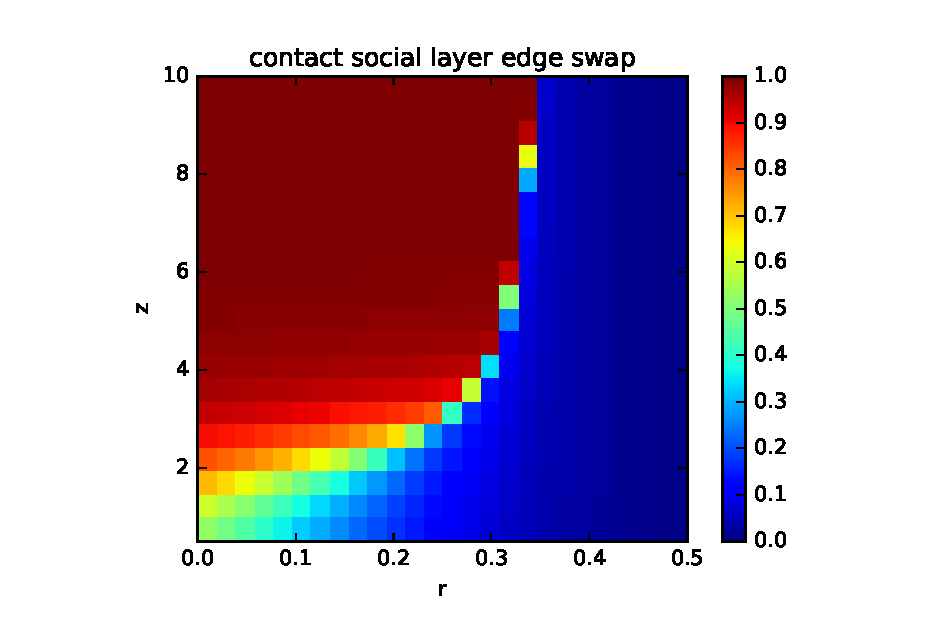
\includegraphics[width=0.7\textwidth]{figures/hetero_edge_swap_ER}
\caption{Phase plane with dependency network = edge swap of ER, contact threshold.}
\end{figure}
Very similar to situation without social network N.B. no Goldilocks.

\end{frame}


\begin{frame}{Contact Awareness: Node swap ER}
\begin{figure}
\centering
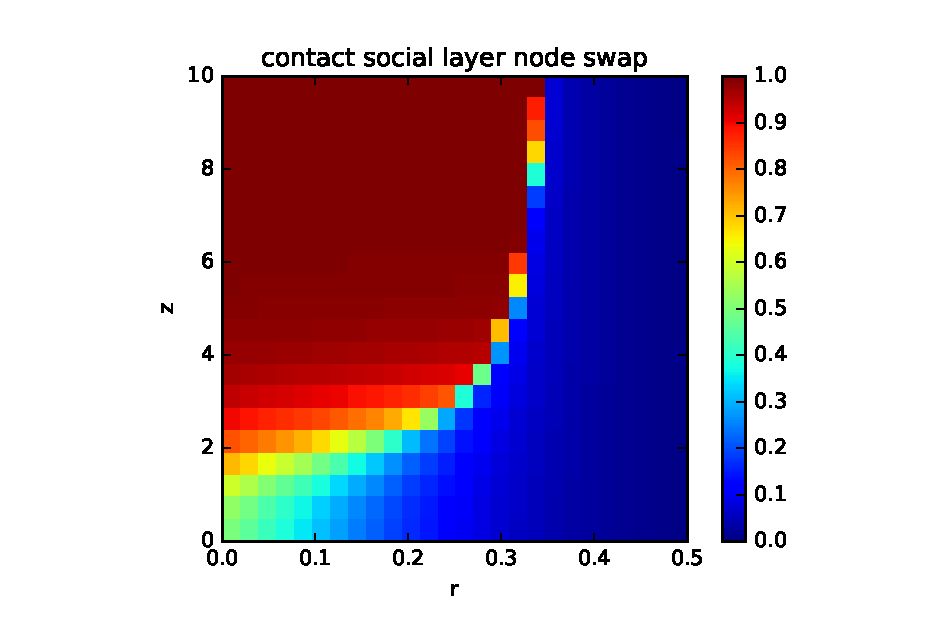
\includegraphics[width=0.7\textwidth]{figures/hetero_node_swap_ER}
\caption{Phase plane with dependency network = node swap of ER, contact threshold.}
\end{figure}
Very similar to situation without social network N.B. no Goldilocks.

\end{frame}


\begin{frame}{Contact Awareness: ER Dependency, PP Social}
\begin{figure}
\centering
\includegraphics[width=0.7\textwidth]{figures/hetero_edge_swap_pp}
\caption{Dependency = ER, Social = PP, contact threshold.}
\end{figure}
Very similar to situation without social network N.B. no Goldilocks.

\end{frame}

\begin{frame}{Contact Awareness: PP Dependency, ER Social}
\begin{figure}
\centering
\includegraphics[width=0.7\textwidth]{figures/hetero_edge_reverse_swap_pp}
\caption{Dependency = PP, Social = ER, contact threshold.}
\end{figure}
\end{frame}


\begin{frame}{Contact Awareness: node swap, PP Dependency, PP Social}
\begin{figure}
\centering
\includegraphics[width=0.7\textwidth]{figures/hetero_node_swap_pp}
\caption{Dependency = PP, Social = ER, contact threshold.}
\end{figure}
Limited extent of infection appears again when PP swaps nodes.
\end{frame}



\begin{frame}{Summary}
\begin{itemize}
\item There is a \textbf{phase transition} between very little coordination to extensive, population wide coordination at critical values of \emph{social awareness} and \emph{degree of dependency}
\item Highly socially aware agents are safe against decoupling of social and dependency network
\item Community networks are inflexible against solving structured problems whose dependencies do not correspond to the same community structure. (\emph{Limited horizon of infection})
\item Node swap is more dangerous because it disconnects agents with a high degree of dependency.
\item Future extensions: different threshold distributions, different network topologies, adaptive social networks.
\end{itemize}
\end{frame}

\begin{frame}[standout]
Major thanks to my supervisors Stephen Cassidy and Stephen Brewis @BT and Renaud Lambiotte and Andrew Mellor @Oxford.
\end{frame}
\begin{frame}[t,allowframebreaks]
\printbibliography
\end{frame}

\end{document}
